\chapter{Information Extraction}

			\section{Problem Definition}

			\par
			We first define what constitutes a rumor.As per \cite{difonzo2007rumor} a rumor is defined as -
			\begin{center}
					A rumor is a controversial and fact-checkable statement.
			\end{center}
			We make certain observations related to the above definition:-
			\begin{itemize}
				\item Fact-checkable: It means that one can verify the correctness given the concrete evidence for the same.Statements for which truth value will be determined in future are not included.
				
				\item 
				Disputable: People will not accept and will question the belief discussed in the information.
			\end{itemize}
			Any statement will includes a reference to a statement which has the above 2 properties can be also considered as rumor.
			\\
			\par
			Most of the work done above in the context of rumor detection considers the data using only it's lexical and syntactic features.For example, work done in \cite{zhao2015enquiring} treats tweets using the Bag-of-Words model to calculate the tweet similarity.For the problem of rumor detection it is necessary to identify the subjects that the rumor is spreading.Using the Bag-of-Words model,we don't have any sufficient information to identify the subject(s) that is/are being discussed  in tweet data involved. The accurate subject identification of tweets however is a challenging task since the limited number of tokens in a post often implies a lack of sufficient	contextual information.There is a certain need to analyze the problem by identifying its semantic features.\\
		
			\par
			The problem is formulated as follows.Given a set of tweets,we need to group them into rumor clusters.Each cluster is identified by the subject discussed in the rumor.Then we enrich the semantic context of each cluster by extracting subjects contained in them.After this step,rumor analysis of each cluster is to be done to indicate the probability that it represents a rumor.The subjects which are extracted using Part-of-Speech tags are used to extract semantic information from the tweets.The semantic information is then used to cluster the tweets as a similarity measure.
			\\
			\par
			The below diagram shows the overall flow of the working of the system proposed.\\
			\begin{figure}[H]
				\centering
				\begin{minipage}{1\linewidth}
					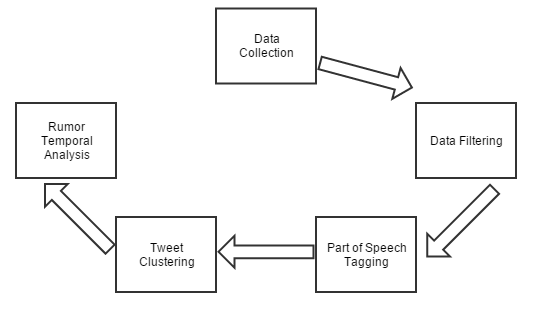
\includegraphics[width=\linewidth]{images/block.png}
					\captionof{figure}{Flow diagram}
					\label{img1}
				\end{minipage}
			\end{figure}
			
		\clearpage	
			
		\section{Terminology}
		
		We first define some Twitter specific terms that will be used:-
		
		\begin{itemize}
			\item Tweet - Each message written on Twitter is called a tweet.
			\item Feed - A feed is any constantly-updating list of tweets or other updates, usually sorted chronologically with the most recent updates appearing at the top.
			\item Follower - On Twitter, you follow another user to see his or her updates on your Twitter home page.
			\item Mention - Twitter allows user to mention other user in a tweet using @ symbol.
			\item Hashtag - Using \# symbol a user can enrich the subject being discussed in the tweet.  
			\item Retweet - Using retweet we can make someone else's tweet appear in stream of our followers.
		\end{itemize}	
					
		\section{Data Collection}
		\par
		The tweets are collected using the Twitter Streaming API which provides 1\% sample of the real-time tweets.We use the data available from Twitter for the month of July 2015.Given the huge volume of the data,the tweets are stored into a NoSQL MongoDB database in JSON format.A NoSQL (originally referring to "non SQL" or "non relational") database provides a mechanism for storage and retrieval of data which is modeled in means other than the tabular relations used in relational databases.Storing in the JSON format allows the meta-data to be updated over the time to add new features to the tweet data as well as enable efficient retrieval of large amount of data.The JSON data is then exported to HDFS for Map-Reduce operations on this large scale data.
		\\
		\par
		The current dataset is limited to tweets which are written only in the English language.The information contained in the tweet meta-data is used to select only the English tweets.The data is filtered to remove the tweets which are written in multiple lines.This is done to facilitate processing on HDFS which considers one line as a single record.As the number of tweets having multiple lines is a small fraction of the total tweets,it is assumed that removing these does not impact the correctness of further operations.The tweets were also more or less evenly divided between each day of week, with each day having somewhere between 14\% and 15\% of the tweets. Similarly, the tweets were almost evenly divided between each hour, with each having somewhere between 3\% and 5\% of the tweets.The overall distribution of the tweets posted per day for the month of July 2015 of the 1\% dataset is shown below. 
		
			\begin{figure}[H]
				\centering
				\begin{minipage}{.7\linewidth}
					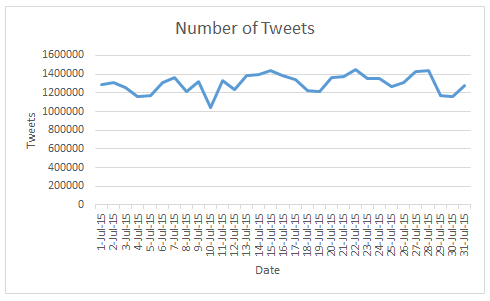
\includegraphics[width=\linewidth]{images/num_tweets.png}
					\captionof{figure}{Number of Tweets}
					\label{img_nt}
				\end{minipage}
			\end{figure}

		\section{Data Filtering}
		\par The set of tweets collected is divided into two sets - signal tweet and non signal tweet.Signal tweets are those which contain enquiry pattern such as "really?","is it true" as identified in \cite{zhao2015enquiring}.These signal tweets are used as signal element to identify a rumor.All others tweets other than enquiry tweets are collected into the non signal tweet set.
		This is done to identify the first set of signal that may be used to indicate that a tweet may be a rumor.As per figure \ref{img_nt} we have seen that the number of tweets per day is very large and the average is around 1.3 million tweets per day.To process such data,we need certain type of distributed computation to scale up the processing time and get results within a minimum stipulated time.We have used Hadoop framework to process this "big" data.Hadoop used HDFS as the filesystem to store files i.e. the tweet data in current context.The Map-Reduce framework is then used to filter the tweets wherein the work is distributed to multiple machines in the cluster and partial results are then aggregated to form a unified dataset of filtered tweets.  
		
		
		\section{Part-Of-Speech Tagging}
		A Part-Of-Speech Tagger (POS Tagger) is a piece of software that reads text in some language and assigns parts of speech to each word (and other token), such as noun, verb, adjective.The current approach uses POS tagging to extract syntactic features from each tweet rather than the lexical model used in previous works.The syntactic features will be later used to derive semantic information about each subject discussed in the tweet cluster.		Standard POS tagging tools are used to extract POS tags from sentences in long documents.Tweets are online conversations which are short and it's word usage is different than of long text documents.Standard POS tagging tools are trained on data sets of large words,hence do not work on tweets.A specialized tool for tweets is needed for perform POS tagging efficiently.So an existing efficient and specialized Twitter POS tagging tool \cite{gimpel2011part} is used for extracting  POS features.The tool decomposes the tweets into various components such as proper noun,common noun,verb,adjective,adverb and interjection.Some Twitter specific POS tags such as hash tag,user-mention,URL and emoticon are also retrieved.

		\par For example, the following tweet
		\begin{center}
		 "RT @brownjenjen : Ben Affleck denies affair rumors
		\#rumor http://t.co/qwrfe"
		\end{center} 
		\par is decomposed in POS tags as follows:-
		
		
\begin{table}[H]
	\centering
	\begin{tabular}{@{}|l|l|@{}}
		\toprule
		RT                & Re-tweet         \\ \midrule
		@brownjenjen        & At-mention       \\ \midrule
		:                 & Discourse marker \\ \midrule
		Ben               & Proper Noun      \\ \midrule
		Affleck           & Proper Noun      \\ \midrule
		denies            & Verb             \\ \midrule
		affair            & Common Noun      \\ \midrule
		rumors            & Common Noun      \\ \midrule
		\#rumor           & Hashtag          \\ \midrule
		http://t.co/qwrfe & URL              \\ \bottomrule
	\end{tabular}
	\caption{Tweet Part-of-Speech Tagging}
	\label{my-label}
\end{table}




\section{Tweet Clustering}
This process involves dividing a set of tweets into subsets, where elements in each subset are considered related by some similarity measure.It is very rare that tweets which contain different subjects will contain any similarity on a semantic basis.Using a string similarity measure may lead  to a spurious similarity for tweets even if they are not related.So the current approach avoids use of a string similarity measure and instead represents each tweet by proper nouns and URLs contained in it.These are obtained by the POS tagging step done earlier.The number of similar proper nouns and URLs are used a measure of similarity.
\\
\par
Each tweet is added as a node in the graph.An edge is added between two tweets only if they represent some common subject i.e. proper noun/URL.The weight of the edge determines the degree of similarity which is number of matching POS tags.Any POS tag that is matched is assigned a score of 1.The edge accumulates the scores of individual matching POS tags.An undirected graph of tweets is built by including an edge joining any tweet pair with a similarity score of at least 2.
This is done to ensure that the rumors clusters are accurate.The accuracy of the clusters is determined by the subject discussed within them but also by its context.It may happen that one subject is being discussed with two different contexts in the same temporal dimension.For example,"Obama" may be discussed related to two other subjects such as "nuclear deal" and "war".It is necessary to form two candidate rumor clusters separately for each of them.By adding an edge only when similarity score is 2,such dataset will have two clusters - one related to "Obama" POS tags with "nuclear deal" related POS tags and the other with "Obama" POS tags with "war" related POS tags.This splitting of clusters also allows each cluster to be analyzed independently of each other.This improves the coherent quality of each cluster as each of them has the exact context discussed and does not mix tweets with other context.      
\\
\par
A connected component in an undirected	 graph is a group of vertices, every pair of which are reachable from each other through paths.The connected components in such a graph will contain the tweet cluster which discuss a common subject.Next,we calculate the summary features of each cluster by including the POS tags which occur in more than 25\% of the tweets in the cluster.This step ensures that only the subjects that are actively being discussed will be brought in the tweet cluster summary.The summary statement consisting of POS tags is now compared with each tweet in the non signal cluster set to increase the cluster size.	  
\\
\par
The entire algorithm is outlined below.

\begin{algorithm}[H]
	\caption{\em Tweet clustering algorithm from Part-of-Speech tags - Single Day }
	\textbf{Input:} Raw tweets from Twitter 1\% sample dataset \\
	\textbf{Output:} Clusters of candidate rumors 
	%\begin{minipage}{\linewidth}
	\begin{algorithmic}[1]	 	
		\FOR{ All tweets in dataset }
		\IF{Tweet contains enquiry pattern} 
		\STATE{Add tweet to signal tweets set} 
		\ELSE 
		\STATE{Add tweet to non signal tweets set} 
		\ENDIF
		\ENDFOR    
		
		\FOR{ All tweets in the signal set}
		\STATE Add tweet as node in graph 
		\STATE	 Extract Part-Of-Speech tags from each tweet 
		\STATE	 Assign proper noun and/or URL as features for each tweet
		\STATE	 Compare with rest of the signal tweets
		
		\IF{Number of features matching is greater than or equal to 2} 
		\STATE{ Add edge between the tweets }
		\ENDIF
		\ENDFOR
		\STATE Get connected components from the graph
		\IF{ Size of connected component is less than 2 }
		\STATE Discard connected component
		\ELSE
		\STATE Consider connected component as a candidate rumor cluster
		\ENDIF
		\FOR { Each candidate cluster}
		\FOR { Each tweet in the cluster}
		\IF {Feature of tweet is contained in more than 25\% percent of the tweets in the cluster}
		\STATE Add feature to summary feature set of the cluster 
		\ENDIF
		\ENDFOR
		\ENDFOR
		\algstore{testcont} 
	\end{algorithmic}
	\addtocounter{algorithm}{-1}%% <===
\end{algorithm}

\begin{algorithm}[H]
	\caption{\em Tweet clustering algorithm from Part-of-Speech tags - Single Day}
	\begin{algorithmic}[1]
		\algrestore{testcont}  
		\FOR { Each candidate cluster}
		\FOR { Each tweet in the non signal tweets}
		\IF{ Number of matching features between candidate cluster summary and the non signal tweet is greater than or equal to 2 }
		\STATE Add tweet to candidate rumor cluster 
		\ELSE
		\STATE Discard the tweet for further processing 
		\ENDIF 
		\ENDFOR
		\ENDFOR 
	\end{algorithmic}
	%\end{minipage}
\end{algorithm}

		\section{Results}
		To process such large data in a distributed manner, the algorithms were executed out on a Hadoop cluster having 15 nodes.The data filtering results for signal tweets that were carried out are explained below.
		
		\begin{figure}[H]
			\centering
			\begin{minipage}{.7\linewidth}
				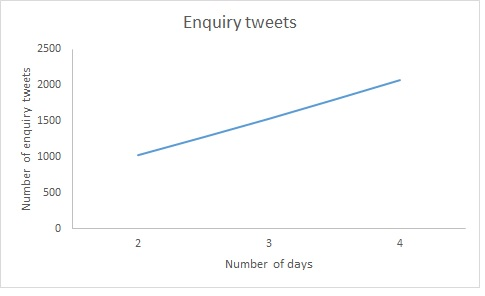
\includegraphics[width=\linewidth]{images/result1new.jpg}
				\captionof{figure}{Days vs Signal Tweet Size}
				\label{img1}
				\end{minipage}
		\end{figure}
		
		Figure \ref{img1} shows the number of enquiry tweets collected over days.The number of enquiry tweets is directly proportional to the size of the dataset.This concludes that everyday there exists a proportion of the users whose post enquiry tweets.This linear increase also proves that each day  there is more or less a fixed amount of Twitter chatter which consists of the portion of signal tweets.
				
		\begin{figure}[H]
					\centering
					\begin{minipage}{.7\linewidth}
						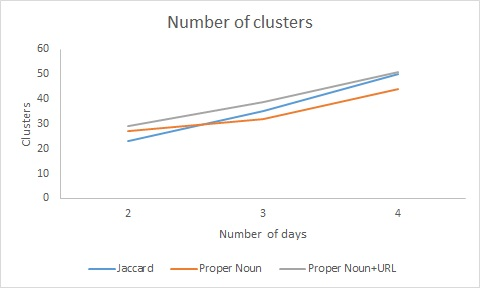
\includegraphics[width=\linewidth]{images/result2new.jpg}
						\captionof{figure}{Number of clusters}
						\label{img2}
						\end{minipage}
		\end{figure}
		
			Figure \ref{img2} shows that the number of clusters we get using tweet similarity measure as Jaccard distance is similar to the number of clusters we get using the proper noun POS tweet similarity measure.The proper noun+URL POS tweet similarity measure provides the best performance in all cases.Thus,we stick to this measure for all further operations.
						
		\begin{figure}[H]
							\centering
							\begin{minipage}{.7\linewidth}
								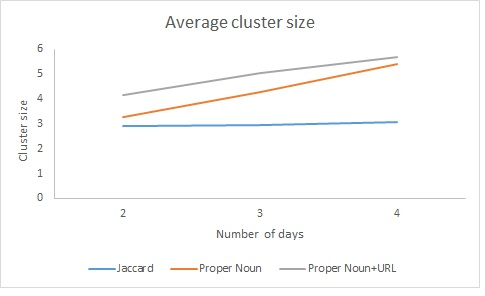
\includegraphics[width=\linewidth]{images/result3new.jpg}
								\captionof{figure}{Average cluster size}
								\label{img3}
								\end{minipage}
		\end{figure}
		
		Figure \ref{img3} shows the average cluster size for varying amount of tweet data.The average cluster size does not increase for Jaccard distance as larger datasets containing the same concept contains tweets which will contain diverse words. The diversity of the words involved in larger datasets will reduce the Jaccard similarity between tweets leading to small clusters being formed.When using POS tags, diverse words wont affect the result as they are not taken into account when determining the cluster similarity.In fact more the data, POS tag approach will lead to bigger clusters being formed.If we add URLs extracted from the POS tag in addition to proper noun, we get more bigger clusters as many tweets which contain a rumor which share a URL which contains more information about the fact being claimed.
								
		\begin{figure}[H]
									\centering	
									\begin{minipage}{.7\linewidth}
										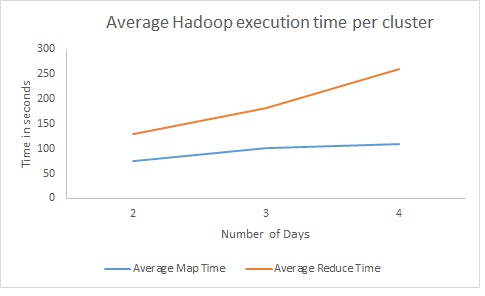
\includegraphics[width=\linewidth]{images/result4new.jpg}
										\captionof{figure}{Hadoop execution time}
										\label{img4}
										\end{minipage}
		\end{figure}
										

		While increasing the dataset shows improvement in the number of clusters and the average cluster size as shown in the Figures  \ref{img2} and \ref{img3},the corresponding time required to process the non signal tweets to be assigned to a signal cluster also increases as shown in figure \ref{img4}.In fact,the time required for Reduce operation starts to increase non-linearly.This metric is crucial when we need to detect rumors as quickly as possible.
		
		\section {Summary}
		
		This chapter has focused on the defining the rumor detection problem in a broad context.The data collection and filtering for the rumor detection purpose has been explained in detail.The semantic information extraction from a single day of Twitter data and its results using Hadoop cluster have been examined.We have also found that Proper Noun+URL Part-of-Speech similarity measure perform the best when clustering the tweets.In the next chapter,we deal with combining the individual Hadoop results of single days and performing rumor analysis.
		
	